\documentclass[conference]{IEEEtran}
\usepackage{cite}
\usepackage{amsmath,amssymb,amsfonts}
\usepackage{graphicx}
\usepackage{url}

\begin{document}

\title{Algebra Assignment \\
CSE 625 - Project 2}

\author{\IEEEauthorblockN{Chequer Cabrera, Diego Emilio}
\IEEEauthorblockA{\textit{Student ID: 5412035} \\
\textit{d0cheq01@louisville.edu}}
\and
\IEEEauthorblockN{lastname, firstname}
\IEEEauthorblockA{\textit{Student ID: <ID>} \\
\textit{student@louisville.edu}}}

\maketitle

\begin{abstract}
TODO: Write the abstract once the project results are complete.

\end{abstract}

\section{Introduction}

TODO: Introduce the problem, project goals, and approach.

\section{Original Sequential Baseline}
\label{sec:original-baseline}

\subsection{Measurement Procedure}
The implementation was developed and small tests were measured on \texttt{louie}, a KVM virtual
machine exposing four logical CPUs with an Intel Core i3-12100F
with 16GiB of RAM.
Compilation used GNU g++ 14.2.0, CMake 3.31.6, and Release flags
\texttt{-O3 -DNDEBUG -std=gnu++20}.

The tested square matrix dimensions were $N=64$, $128$, and $256$.
For each dimension, the executable was configured and built once before
three separate measured executions. Each execution used seed 123456 and
the field of order $11^3=1331$, with defining polynomial $x^3+x+4$.
The build command and the first measurement command used for $N=256$
are recorded below as an example, other dimensions just substitute 
the size in the \texttt{-DALGEBRA\_ASSIGNMENT\_SIZE} option and the log file name.

\begingroup
\scriptsize
\begin{verbatim}
cmake -S . -B build \
  -DCMAKE_BUILD_TYPE=Release \
  -DALGEBRA_ASSIGNMENT_SIZE=256 \
  && cmake --build build --parallel

/usr/bin/time -v \
  ./build/src/algebra_determinants \
  2>&1 | tee original-256-run1.log
\end{verbatim}
\endgroup

Only the executable was timed, not the build. The combined output retained
the field metadata, determinant coefficients, correctness check, application
phase timings, and GNU Time resource measurements. All nine runs returned
exit status zero and verified $\det(AB)=\det(A)\det(B)$. For each dimension,
the determinant coefficients agreed across all three repetitions.

\subsection{Runtime and Peak Memory}
Table~\ref{tab:original-baseline} reports the median GNU Time elapsed wall
time, the median application-reported total, and the largest peak resident
set size among the three repetitions. 
The application total uses its own steady-clock interval.

\begin{table}[tb]
\centering
\caption{Original sequential baseline over three runs per dimension}
\label{tab:original-baseline}
\begin{tabular}{rrrr}
\hline
$N$ & Wall (s) & App total (s) & Peak RSS (MiB) \\
\hline
64 & 0.15 & 0.151263 & 4.684 \\
128 & 1.10 & 1.102611 & 7.121 \\
256 & 8.73 & 8.728325 & 17.637 \\
\hline
\end{tabular}
\end{table}

Application total times ranged from 0.147525 to 0.151736~s at $N=64$,
1.098483 to 1.110965~s at $N=128$, and 8.640466 to 8.730073~s at $N=256$.
Doubling the dimension from 128 to 256 increased the median application
total by approximately 7.92 times, consistent with the cubic arithmetic
work of matrix multiplication and elimination.

Table~\ref{tab:original-phases} separates multiplication from the three
determinant computations. Each timing column is summarized independently.
For $N=256$, the median combined time for calculating all three 
determinants was 4.273438 seconds, while matrix multiplication took 4.418723 seconds. 
This indicates that multiplication took slightly longer than the three determinant calculations combined.

\begin{table}[tb]
\centering
\caption{Median original phase times in seconds}
\label{tab:original-phases}
\begin{tabular}{rrrrr}
\hline
$N$ & Product & $\det(A)$ & $\det(B)$ & $\det(C)$ \\
\hline
64 & 0.0797 & 0.0227 & 0.0230 & 0.0228 \\
128 & 0.5468 & 0.1794 & 0.1805 & 0.1801 \\
256 & 4.4187 & 1.4143 & 1.4193 & 1.4212 \\
\hline
\end{tabular}
\end{table}

These results establish the original runtime and memory baseline on the
local host. Per-run measurements, summary statistics, and environment metadata
are retained in the repository alongside the raw logs.

\subsection{Function-Level Profile}
\label{sec:original-profile}
A separate run at $N=256$ used GNU gprof 2.44, adding \texttt{-pg -g} during
compilation and \texttt{-pg} during linking. The program retained Release
optimization, the same seed, and the original arithmetic. It verified the same
determinants and multiplicative identity. Its profiling data and text report
were generated with the following commands:

\begingroup
\scriptsize
\begin{verbatim}
./build/src/algebra_determinants \
  > original-256-profile-run.log
gprof -b ./build/src/algebra_determinants \
  gmon.out > original-256-profile.txt
\end{verbatim}
\endgroup

Fig.~\ref{fig:original-profile} shows the flat profile's sampled self-time
shares. Self time excludes separately reported callees~\cite{gprof-flat}.
Matrix multiplication accounted for 49.71\%, the determinant function for
35.19\%, and polynomial division/remainder for 12.13\%. The profiler recorded
50,233,382 calls to the polynomial \texttt{divmod} routine. The small remaining
shares were attributed to the \texttt{\_init} symbol and random-generator state
refresh.

\begin{figure}[tb]
\centering
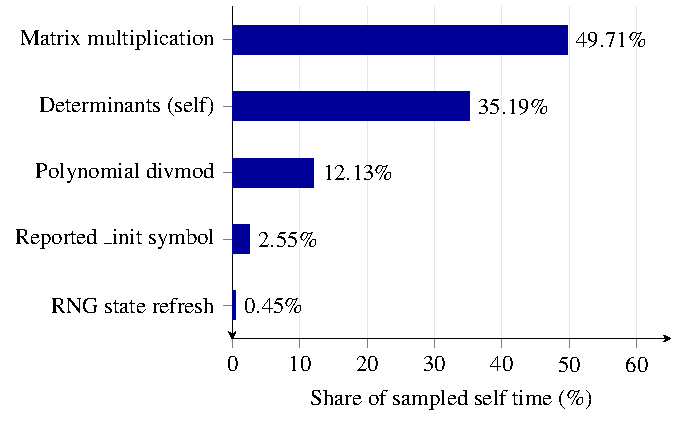
\includegraphics[width=\columnwidth]{figures/original-profile.pdf}
\caption{Reported sampled self-time shares for the optimized, instrumented
$256\times256$ original run. Values describe profiler samples, not wall-time
fractions; inlined arithmetic is attributed to its enclosing function.}
\label{fig:original-profile}
\end{figure}

\section{Cached Sequential Comparison}
\label{sec:cached-comparison}
Both backends were measured again on the same host with the same Release
compiler flags, seed, and field as Section~\ref{sec:original-baseline}.
Each point represents three separate sequential processes, so the arithmetic
caches begin empty for each run. The whole-workload application interval includes
generation, matrix multiplication, the three determinants, and cache creation
and filling; it ends before static-cache destruction. Peak resident set size
(RSS) includes the cache. Builds and profiling were excluded from these timings.
All executions returned successfully, verified the determinant identity, and
matched the original determinant coefficients at their dimension.

Fig.~\ref{fig:backend-comparison} compares median application totals, the
ratio of original to cached medians, and the largest peak RSS among the three
runs. The runtime axis is logarithmic. At $N=64$, the median speedup was only
1.10 times, while cached peak RSS increased from 4.68 to 10.48~MiB. At $N=256$,
the median speedup was 9.76 times and cached peak RSS decreased from 17.62 to
10.93~MiB. These results reflect both compact element storage and arithmetic
memoization; they do not isolate either contribution.
At $N=512$, the respective median totals were 70.56 and 3.44~s (20.50 times),
and peak RSS was 59.61 and 12.47~MiB.

\begin{figure}[tb]
\centering
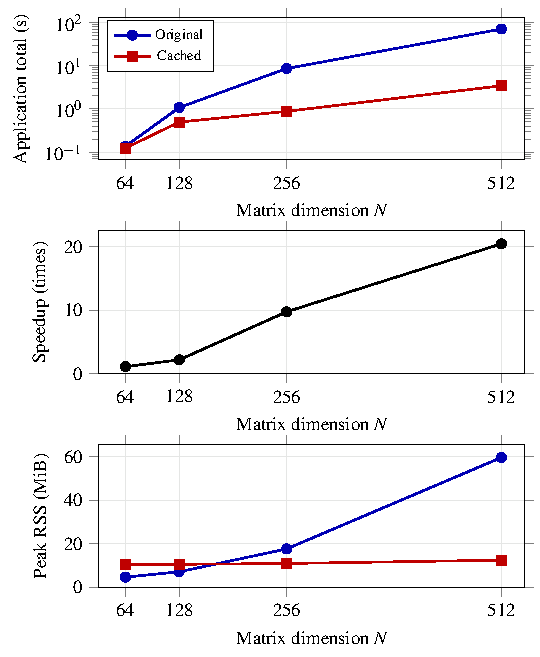
\includegraphics[width=\columnwidth]{figures/backend-comparison.pdf}
\caption{Sequential backend comparison. Times are three-run medians, speedup is
the ratio of those medians, and RSS is the largest peak across the three runs.}
\label{fig:backend-comparison}
\end{figure}

The small-input memory increase is consistent with the implementation's fixed
cost: the two binary-operation tables alone hold $2\cdot 1331^2$ two-byte IDs,
approximately 6.76~MiB, before the element catalog and other allocations.
As matrix size grows, the cached representation stores each matrix element as
a two-byte ID. This helps explain the observed reversal in RSS; these figures
do not establish a precise break-even dimension.

The product executes before the determinants and shares the same cache with
them. Consequently, determinant phase timings include the effect of entries
filled earlier and are not cold-cache determinant measurements. More cache
filling during the larger product may explain why the median sum of cached
determinant times decreases from $N=128$ to $N=256$, but occupancy was not
measured. The runs were collected in a fixed backend order on one virtualized
host; three repetitions at each size do not establish assignment-scale or MPI
performance.

\subsection{Cached Function-Level Profile}
The cached workload at $N=256$ was profiled separately with the same optimization
and gprof instrumentation described in Section~\ref{sec:original-profile}.
Ten fresh-process profiles were combined to increase the sample count; the
reported call counts and sampled seconds are totals across all ten executions.
The flat profile accounted for 7.82~s of sampled self time at a 0.01~s sampling
interval. Fig.~\ref{fig:cached-profile} shows the largest reported shares:
matrix multiplication 75.20\%, determinants 13.81\%, and polynomial division
8.70\%. Division remains present because cache misses use original arithmetic.

\begin{figure}[tb]
\centering
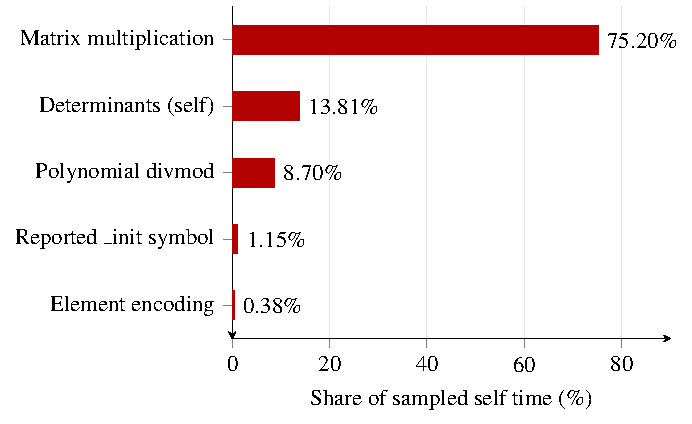
\includegraphics[width=\columnwidth]{figures/cached-profile.pdf}
\caption{Reported sampled self-time shares from ten instrumented, fresh-process
cached runs at $N=256$. Inlined arithmetic is attributed to its caller.}
\label{fig:cached-profile}
\end{figure}

These shares are relative to the sampled time of the cached profile, not a
comparison of absolute costs with Fig.~\ref{fig:original-profile}. Inlining
and sampling affect attribution~\cite{gcc-inline,gprof-sampling}; timing
speedups come from the separate uninstrumented repetitions. The profile's
19,085,010 recorded division calls are summed over ten runs and do not count
operations that were inlined.


\begin{thebibliography}{00}
\bibitem{gprof-flat} GNU Binutils, ``The Flat Profile,'' GNU gprof manual. [Online]. Available: \url{https://sourceware.org/binutils/docs/gprof/Flat-Profile.html}
\bibitem{gprof-sampling} GNU Binutils, ``Statistical Sampling Error,'' GNU gprof manual. [Online]. Available: \url{https://sourceware.org/binutils/docs/gprof/Sampling-Error.html}
\bibitem{gcc-inline} GNU Project, ``An Inline Function is As Fast As a Macro,'' Using the GNU Compiler Collection. [Online]. Available: \url{https://gcc.gnu.org/onlinedocs/gcc/Inline.html}
\end{thebibliography}

\end{document}
